\documentclass[a4paper,11pt]{article}

\usepackage[utf8]{inputenc}
\usepackage{amsmath}
\usepackage{amsfonts}
\usepackage{dirtytalk}
\usepackage{physics}
\usepackage{biblatex}
\usepackage{hyperref}
\usepackage[ignoreunlbld]{refcheck}
\usepackage{booktabs}
\usepackage{multirow}
\usepackage{longtable}
\usepackage{float}
\usepackage[font=normalsize]{caption}
\usepackage{graphicx}
\setkeys{Gin}{width=.8\textwidth}
\graphicspath{ {./images/} }
\usepackage{indentfirst}
\addbibresource{ref.bib}


\font\Bbb=msbm10 at 11pt
\def\QQ{\mbox{\Bbb Q}}
\def\RR{\mbox{\Bbb R}}
\def\ZZ{\mbox{\Bbb Z}}
\def\NP{{\cal NP}}

\newtheorem{definition}{Definition}
\newtheorem{lemma}{Lemma}
\newtheorem{proposition}{Proposition}
\newtheorem{remark}{Remark}
\newtheorem{theorem}{Theorem}


\newenvironment{proof}
{\begin{trivlist} \item[] {\bf Proof.\ }}{\hfill$\Box$ \end{trivlist}}

\title{Using Sensitivity Analysis from Stochastic Programs to Inform Marketing Decisions}

\author{Congzheng Liu\thanks{Department of Management Science,
Lancaster University, Lancaster LA1 4YX, UK.
Email: {\tt \{c.liu19,a.n.letchford,i.svetunkov\}@lancaster.ac.uk}}
\and Adam N.\ Letchford$^*$ \and Ivan Svetunkov$^*$} % end author list

\date{8th August 2020}

\begin{document}

\maketitle

\begin{abstract}
Although marketing and inventory control are normally different functions in a business, it is obvious that both forecasting errors and marketing interventions are relevant to ordering or production decisions. In this paper, we describe a framework which enables one to use information gained in the inventory control phase to improve the marketing phase. In detail, we consider a single-period multi-product newsvendor problem, which we model as a two-stage stochastic linear program with simple recourse. We then use sensitivity analysis to estimate the marginal increase/decrease in expected profit that would arise from improvements in forecasting or marketing interventions.
\\*[2mm]
{\bf Keywords:} marketing; inventory control; forecasting; newsvendor problems; stochastic programming
\end{abstract}

\section{Introduction}
Inventory control has always been treated as an important part of Operations Research and Management Science \cite{Po02,SPP98,Zi00}. In this paper, we consider a production planning problem, which can be viewed as a kind of single-period multi-product
Newsvendor problem (MPNP)\cite{D98,TTV12}.

In general, MPNP considers the manufacturing and/or retailing procedure in a company with multiple products \cite{SPP98}. Regarding to the natures of applier, the constraints in MPNP could be manufacturing abilities, storage capacities or funding powers, etc. Here, we refer all as resources for convenience. In this paper, we assume the applier is a manufacturer, and we use manufacturing terms in formulation. In this case, the goal of MPNP is to decide the optimal quantities of each product to be manufactured regarding to a given cost function, while satisfies all dimensions of resource at the same time \cite{BDR12}. The cost function is similar to the classical Newsvendor problem \cite{Ch12}, where the expected cost is formed by \emph{over-stocking} cost, \emph{under-stocking} cost and stochastic demand.

The classical approach to MPNP is sequential. First, demand of products are estimated by experts in field of forecasting. Then, the quantities deciding process is considered, which is an optimisation problem usually handled by computational experts. This two stage method is usually called disjoint method, in contrast with integrated method, which usually derive decision directly from data \cite{Sc58}. 

In this paper, we concentrate on the second stage of the disjoint method. Specifically, we focus on post-optimisation phase where one can analysis how \emph{new effort} could alter our decision, referred as \say{sensitivity analysis (SA)} in field of optimisation \cite{D98,Ga03,Va20}. We use linear programming (LP) with generated scenario set to approximates the stochastic feature of MPNP, and use a non-standard SA approach to inform marketing decision. Unlike the standard approach that determine the effect of changes in the objective function coefficients or the right-hand sides of the constraints \cite{DT06}, we use it to estimate the effect of changes in the moments (e.g., means, variances and covariances) of the demand distribution. 

This method is stable and very efficient. We don't need to resolve the optimisation problem when demand alters, but apply our sensitivity analysis results directly as long as the changes in allowable interval. Moreover, Our approach can also be view as an attempt to create a \say{feedback loop}, so that the output from the optimisation phase is used to guide choices about whether it would help to obtain more accurate estimates of the demand distribution (e.g., by market research), or even to take action to change the distribution (e.g., by promotions).

The rest of this paper is organized as follows. Section \ref{se:lit} presents works in previous literature. Section \ref{se:model} specificates the model. Section \ref{se:sensitivity} contains the sensitivity analysis with an example. Section \ref{se:extensions} presents extensions to the analysis.

%%%%%%%%%%%%%%%%%%%%%%%%%%%%%%%%%%
\section{Literature Review}
\label{se:lit}
MPNP is one extension of classical Newsvendor problem (NVP). Here we assume readers are familiar with the basic of NVP. The reader looking for more background knowledge is directed to the books \cite{Ch12,Po02,SPP98}.

\subsection{Multi-product Newsvendor Problem}
\label{sub:lit_mpnp}
In the traditional MPNP, found in \cite{HW63,NS84}, a manufacturing company is interested in determining quantity $x_j$ for product $j (j=1,\dots,n)$ to satisfy the demand. For each product, the demand is assumed to be stochastic, defining as ${\tilde d}_j$ with known distribution (could also be partial distribution). Yet, products left over lead to \emph{over-stocking} opportunity cost $c_j^o = c + l_h$ per unit, while shortfall are punished with \emph{under-stocking} opportunity cost $c_j^u = r - c + l_s$ per unit, where $r$ denotes the revenue, $c$ denotes the manufacturing cost, $l_h$ denotes the holding loss, and $l_s$ denotes the shortfall loss, per unit. For a risk neutral manufacturer, the goal is then:

\begin{equation}
    \min \quad \sum_{j=1}^n \mathop{\mathbb{E}} \big( c^o_j \big[  x_j - {\tilde d}_j \big]^+ \, + \, c^u_j \big[ {\tilde d}_j - x_j \big]^+ \big).
\label{eq:uncon}
\end{equation}

It follows that the first order conditions (FOCs) for optimizing (\ref{eq:uncon}) are
necessary and sufficient to determine the optimal quantity of $x_j$ \cite{Ch12}. Based on this, we have:
\[
    x_j^* = F_j^{-1}\left( \frac{c_j^u}{c_j^o+c_j^u} \right),
\]
where $F_j$ is the underlying cumulative distribution function for ${\tilde d}_j$.

In practice, one could add constraints to the optimisation. In general, we set:
\[
    \sum_{j=1}^n s_{ij} x_j \le S_i	\quad (i = 1, \ldots, m),
\]
where $s_{ij}$ denotes the resource required per unit of product $j$ in dimension $i$, and $S_i$ denotes the maximum capacity of resource in dimension $i$. One typical approach to find the optimal order quantity in this setting is using Lagrange multiplier technique  \cite{HW63,LL95}. This technique is straightforward and efficient. Yet, in some practical situations, the optimal $x_j$ will tend to be very small and using this technique could lead to deviations \cite{HW63}. 

Other approaches for constrained MPNP are available in \cite{ALM05,BR93,NS84,ZXH09,Zh10}.


\subsection{Stochastic Linear Programming}
%\label{sub:lit_sto}
Given the nature of underlying uncertainty, one approach to approximate MPNP is stochastic programming \cite{Bea55,D98}. Specifically, we would introduce the two-stage stochastic linear programming with recourse (stochastic LP), which is built from a collection of multi-stage linear programs, each having the same structure but somewhat different data. According to books \cite{HS13,KM76,KWK94,Pf12}, a general stochastic LPs with $S$ scenarios may be regarded as having the following form:
\begin{eqnarray}
    \min	& f ( u ) + \sum_{s \in S} g^s ( v^s )\\
\label{eq:sto_cons1}
	\text{s.t.}    & V_0 u \leq p\\
\label{eq:sto_cons2}
	& V_s u +W_s v^s \leq q^s & (s \in S)\\
	& u, v^s \geq 0 & (s \in S).
\end{eqnarray}
where $f$ and $g$ are linear cost functions, $V$, $W$, $p$ and $q$ are parameters. The vectors $u$ contains the first-stage variables, whose values must be chosen immediately, while the vector $v$ contains all of the variables for subsequent stages. The constraint (\ref{eq:sto_cons1}) involves only first-stage variables and are the same in every scenario, while constraints in (\ref{eq:sto_cons2}) involve variables of second-stage and differ in some respects from scenario to scenario, reflecting uncertainty about the future.

With a finite number of scenarios, this stochastic LP can be viewed as large linear programming model \cite{KW12}. Thus, one can perform SA on the model \cite{AW93,Du95}. The term sensitivity analysis has been used widely. Readers can find applications in books \cite{KCH86,SRA08,STCR04}. In this paper, we refer especially the SA within LPs.

%%%%%%%%%%%%%%%%%%%%%%%%%%%%%%%%%%
\section{Model Specification}
\label{se:model}
We consider following manufacturer model. A company manufactures $n$ products on $m$ machines. Producing one unit of product $j$
takes $t_{ij}$ units of time on machine $i$. Machine $i$ can be used for at most $T_i$ time units. The demand of
product $j$ is a random variable ${\tilde d}_j$ with known distribution. Each unit of product $j$ produced in excess
of demand incurs an over-stocking cost $c^o_j$. Each unit by which demand is unsatisfied incurs an
under-stocking cost $c^u_j$. The company wishes to decide how much of each product to produce, in order
to minimise expected costs $C$. For simplicity, we permit fractions of products to be produced.

It is easy to notice the model with same mathematical structure can also be used to retailing appliers.

\subsection{Problem Formulation}
%\label{sub:problem}
We formulate the problem as follows. For $j = 1, \ldots, n$, let $x_j$ represent the amount of product $j$ produced, then we wish to solve the following stochastic program (SP):

\begin{eqnarray*}
    \min & \sum_{j=1}^n \mathop{\mathbb{E}} \big( c^o_j \big[  x_j - {\tilde d}_j \big]^+ \, + \, c^u_j \big[ {\tilde d}_j - x_j \big]^+ \big) \\
	\text{s.t.}    & \sum_{j=1}^n t_{ij} x_j \le T_i	& (i = 1, \ldots, m) \\
	& x \in \RR_+^n.
\end{eqnarray*}

Following the standard approach \cite{BL11}, we can construct a stochastic LP that approximates the SP. Consider a set $S$ of
scenarios, i.e., realisations of demand obtained from market simulation. We let $d_j^s$ denote the demand for product $j$ in scenario $s$. We also let $y_j^s$ be the number of units over-stocked (if any), and let $z_j^s$ be the number of units under-stocked (if any), respectively, in scenario $s$. The LP is then:
\begin{eqnarray}
\label{eq:obj}
    \min	& \sum_{s \in S} \sum_{j=1}^n \big( c^o_j y_j^s + c^u_j z_j^s \big) \\
	\text{s.t.}    & \sum_{j=1}^n t_{ij} x_j \le T_i	& (i = 1, \ldots, m) \\
\label{eq:over}
	& y_j^s \ge x_j - d_j^s			& (s \in S; \, j = 1, \ldots, n) \\
\label{eq:under}
	& z_j^s \ge d_j^s - x_j			& (s \in S; \, j = 1, \ldots, n) \\
	& x \in \RR_+^n				& \\
	& y^s, z^s \in \RR_+^n			& (s \in S).
\end{eqnarray}

Denote the solution of SP to be $x_P^*$ and the solution of LP to be $x^*$. It has been studied that $x^*$ converges to $x_P^*$ as $|S| \to \infty$. References are available in \cite{G00,KR93,R96}.

\subsection{Effort Formulation}
\label{sub:information}
Two sources of effort are concentrated: 1). \emph{market promotion} that would affect the mean demand. 2). \emph{market research} that would affect the demand variance. Readers can apply same technique on other sources of effort intuitively.

We formulate margin of the effort mathematically, and therefore, determine whether it is worthwhile to promote, or to conduct market research, on particular product. Moreover, for flexible effort, we could decide to what extent should the effort be applied so as to achieve maximum gain.

\subsubsection{Market Promotion}
\label{ss:promotion}
Consider there exists particular promotion method, say, \emph{advertising} with cost $P_{j'}$, that could manually alter the mean demand of a single product $j'$ without changing anything else, ideally. If the mean demand increased by some quantity $\bar{\epsilon}_{j'}$, then the right-hand sides of the corresponding constraints (\ref{eq:over}) and (\ref{eq:under}) would increase by $\bar{\epsilon}_{j'}$. If we denotes $S_{j'}$ to be the set of all scenarios whose constraint is influenced, the margin can be expressed as:
\[
    \Delta \, C_{mj'} = \sum_{s \in S_{j'}} \pi_s^* \bar{\epsilon}_{j'},
\]
where $\pi^*$ denotes the dual price in the field of SA, viewed as the amount that the objective would improve as the right-hand side of the constraint is increased by one unit \cite{D98}. Therefore, one can easily determine whether to apply a promotion by comparing $\Delta \, C_{mj'}$ with the advertising cost $P_{j'}$. Moreover, for some flexible promotion, one may find it useful to construct $P_{j'}$ as a non-decreasing function of $\bar{\epsilon}_{j'}$, and therefore, to obtain the maximum promotion effect by consulting the relationship between $\Delta \, C_{mj'}$ and $P_{j'}$.

In practice, the increase of demand can also be achieved using trade-off by scarifying unit profit, referred as the \emph{discounting}. From the formulation used in this paper, we consider the trade-off between mean demand and under-stocking cost. Readers can find reference in \cite{Ch12,Po02,SPP98} that provides explanation of viewing profit as a part of opportunity cost in under-stocking.

Suppose we have linear price-demand correlation:

\[
    \mu_j = \alpha + \beta c_j^u,
\]
where $\alpha > 0, \beta < 0$ are parameters. Change of under-stocking cost on product $j'$ by $\Delta c_{j'}^u$ will now affect (\ref{eq:obj}), (\ref{eq:over}) and (\ref{eq:under}). In that case, the objective function coefficient and constraint RHS are altered simultaneously.

However, it has been shown very difficult to deal with joint perturbation and compute its allowable range mathematically \cite{SHH14}. Thus, here we only consider the margin of changes while assuming any small changes we proposed are in the allowable range and do not affect optimal basis. 

To derive the margin, we first denote $N_j^o$ as the number of scenarios that incur over-stocking on product $j$ and $N_j^u$ as the number of scenarios that incur under-stocking on product $j$. Therefore, we should have (derivation see Appendix):
\[
    \Delta \, C_{dj'} = N_{j'}^u \beta \big( \Delta c_{j'}^u \big)^2 + \big[ c_{j'}^u N_{j'}^u \beta - c_{j'}^o N_{j'}^o \beta + \sum_{s \in S} z_{j'}^s \big] \Delta c_{j'}^u.
\]
In this case, the applier can use discounting to balance the trade-off, in order to achieve maximum gain. 
\subsubsection{Market Research}
Now suppose there exists particular market research effort that could improves demand estimation. Here, we consider, specifically, the effect on standard deviation reduction. Let $\mu_j$ denote the mean demand for product $j$. To simulate a decrease in standard deviation of demand for product $j$ by $k\%$, we can alter each $d_j^s$ to $\mu_j + (1-k\%) \big( d_j^s - \mu_j \big)$. Accordingly, we should have an equivalence:
\[
\begin{aligned}
    \epsilon_j^s 
    & = \mu_j + (1-k\%) \big( d_j^s - \mu_j \big) - d_j^s\\
    & = k\% \big( \mu_j - d_j^s \big).
\end{aligned}
\]
We express the margin of market research on product $j'$:
\[
    \Delta \, C_{vj'} = \sum_{s \in S_{j'}} \pi_s^* \epsilon_{j'}^s.
\]
Again, we could view both $\Delta \, C_{vj'}$ and research cost $R_{j'}$ as a function of $k$. One can, therefore, inform research decision by consulting the relationship between $\Delta \, C_{vj'}$ and $R_{j'}$.

\section{Sensitivity Analysis: An Example}
\label{se:sensitivity}

We now compute the dual price, reduced cost, as well as the margin with one typical example. Then we consider the two decisions mentioned in Section \ref{se:model}.

\begin{table}[ht]
\caption{Demand Realisations: Example}
\label{tab:demand}
\centering
\resizebox{\linewidth}{!}{
\begin{tabular}{ccccccccccccc}
\toprule
\multicolumn{1}{c}{\textbf{Products}} & \multicolumn{12}{c}{\textbf{Demand Realisations}} \\
\cmidrule(l{3pt}r{3pt}){1-1} \cmidrule(l{3pt}r{3pt}){2-13}
& $s_1$ & $s_2$ & $s_3$ & $s_4$ & $s_5$ & $s_6$ & $s_7$ & $s_8$ & $s_9$ & $s_{10}$ & $s_{11}$ & $s_{12}$\\
\midrule
product $a$ & 200 & 220 & 180 & 190 & 190 & 210 & 240 & 250 & 200 & 190 & 210 & 240\\
product $b$ & 250 & 230 & 200 & 180 & 210 & 210 & 170 & 150 & 180 & 220 & 260 & 260\\
\bottomrule
\end{tabular}}
\end{table}

\begin{table}[ht]
\caption{Demand Realisations: Statistical Summary}
\label{tab:summary}
\centering
\resizebox{0.55\linewidth}{!}{
\begin{tabular}{ccc}
\toprule
 & product $a$ & product $b$\\
\midrule
mean & 210 & 210\\
standard deviation & 22.96 & 35.93\\
median & 205 & 210\\
1st quantile & 190 & 180\\
3rd quantile & 225 & 235\\
\bottomrule
\end{tabular}}
\end{table}

Suppose we manufacture 2 products on 3 machines. Producing one unit of product $a$ requires 4, 7 ,8 units of time on machine $A$, $B$ and $C$, respectively; Producing one unit of product $b$ requires 6, 5, 8 units of time on machine $A$, $B$ and $C$. The capacities of 3 machines are 2200, 2500 and 3500. Over-stocking cost for product $a$ and $b$ are 5 and 7, while under-stocking cost for product $a$ and $b$ are both 6. For the simplicity of demonstration, we only simulate 12 scenarios for demand. Data and statistics are presented in Table \ref{tab:demand} and \ref{tab:summary}.

There are 50 variables in total, $\big\{ x_1,x_2 \big\} \cap \big\{ y_1^1,\dots,y_1^{12},y_2^1,\dots,y_2^{12} \big\} \cap \big\{ z_1^1,\dots,z_1^{12},z_2^1,\dots,z_2^{12} \big\}$, and for each constraint, we assign a slack variable and/or an artificial variable. The problem can be solve easily with linear solver, with optimal $C=3437.14$, $x_1=207.1$, $x_2=210$. Sensitivity reports see Table \ref{tab:sen_var} and Table \ref{tab:sen_con} in Appendix \ref{se:report}.

Now we consider the efforts described in Subsection \ref{sub:information}.

First, we suppose, by market promotion, the mean demand of product $a$ or $b$ could be increased by $\bar{\epsilon}_a$ and/or $\bar{\epsilon}_b$. Regarding the 100\% rule \cite{BHM77}, we have:

\[
\begin{aligned}
    \Delta \, C_{ma} = 
    \begin{cases}
        6 \, \bar{\epsilon}_a, & \bar{\epsilon}_a \geq -2.88,\\
        unpredictable, & \text{otherwise}.
    \end{cases}\\
    \Delta \, C_{mb} = 
    \begin{cases}
        4.29 \, \bar{\epsilon}_b, & \bar{\epsilon}_b \geq -4,\\
        unpredictable, & \text{otherwise}.
    \end{cases}
\end{aligned}
\]

\begin{figure}[htb]
\centering
\caption{Optimal cost vs. Change of mean}
\includegraphics{Example-figure_files/figure-latex/mean-1.pdf}
\label{fig:mean}
\end{figure}

Surprisingly, one may find that promoting mean demand will actually increases manufacturing cost. That is because the ``cost" referred here is ``opportunity cost" \cite{Ch12,Po02}, which is incurred by \emph{not} gaining the benefit associated with the best alternative choice, e.g., the profit could have been earned. As one could notice in sensitivity reports, the time constraint on machine $B$ is binding. Therefore, only promoting mean demand will not leads any gain to the manufacturer, but increases the demand-supply gap, and therefore, increases opportunity cost even more.

Instead, the manufacturer should concentrate on easing the binding constraint, in order to gain more supply power, and therefore meet the demand. Reversely, the manufacturer could also look into anti-promotion methods (if exist), that convert excess demand into cash flow, e.g., ``selling" customer to other manufacturers to get stable cash back.

One can compare these results with simulation outputs in Figure \ref{fig:mean} for verification.

Similarly, if we consider a change of standard deviation on product $a$ or $b$, say, decreasing by $k\%$, we should have margin gain:
\[
\begin{aligned}
    \Delta \, C_{va} = -12.1 \, k_a,\\
    \Delta \, C_{vb} = -22.1 \, k_b,
\end{aligned}
\]
providing the demand remain positive and variance is no less than zero. In this case, we can see that conducting market research may reduce cost. The simulated results are presented in Figure \ref{fig:var}. The manufacturer, therefore, could decide whether or not to use market research and to what extent should the research be used by comparing research cost and the margin gain.

\begin{figure}[htb]
\centering
\caption{Optimal cost vs. Change of variance}
\includegraphics{Example-figure_files/figure-latex/var-1.pdf}
\label{fig:var}
\end{figure}


\section{Extensions}
\label{se:extensions}

We consider one complicated effort intake now, where two correlated parameters are changed simultaneously. Relevant research see \cite{SHH16,XB17}.

Regarding the market promotion effort we presented in Subsection \ref{ss:promotion}, mean of demand can be deliberately increased by some amount $\bar{\epsilon}$, while all other parameters are fix, ideally. Yet, in practice, increase of demand is usually a trade-off by scarifying unit profit. From the formulation used in this paper, we consider the trade-off between mean demand and under-stocking cost. Readers can find reference in \cite{Ch12,Po02,SPP98} that provides explanation of viewing profit as a part of opportunity cost in under-stocking.

Suppose we have linear price-demand correlation:

\[
    \mu_j = \alpha + \beta c_j^u,
\]
where $\alpha > 0, \beta < 0$ are parameters. Change of under-stocking cost on product $j'$ by $\Delta c_{j'}^u$ will now affect (\ref{eq:obj}), (\ref{eq:over}) and (\ref{eq:under}). The LP becomes:

\begin{eqnarray*}
    \min & \sum_{s \in S} \big[ \sum_{j = 1}^n \big( c^o_j y_j^s + c^u_j z_j^s \big) + \Delta c_{j'}^u z_{j'}^s \big]\\
    \text{s.t.}    & \sum_{j=1}^n t_{ij} x_j \le T_i	& (i = 1, \ldots, m) \\
	& y_j^s \ge x_j - d_j^s			& (s \in S; \, j \neq j') \\
	& y_{j'}^s \ge x_{j'} - d_{j'}^s - \beta \Delta c_{j'}^u           & (s \in S)\\
	& z_j^s \ge d_j^s - x_j			& (s \in S; \, j \neq j') \\
	& z_{j'}^s \ge d_{j'}^s + \beta \Delta c_{j'}^u - x_{j'}        & (s \in S)\\ 
	& x \in \RR_+^n				& \\
	& y^s, z^s \in \RR_+^n			& (s \in S).
\end{eqnarray*}
Furthermore, we can denotes $N_j^o$ as the number of scenarios that incur over-stocking on product $j$ and $N_j^u$ as the number of scenarios that incur under-stocking on product $j$.

It has been shown very difficult to deal with joint perturbations on both objective function coefficient and constraint RHS mathematically \cite{SHH14}. Thus, here we only consider the margin of changes while assuming any small changes we proposed are in the allowable range. 

To visualise our procedure, we consider again the two products example in Section \ref{se:sensitivity}, with $\alpha = 270, \beta = -10$. Higher dimension problem can be solve with same procedure, accordingly. Recalling the results from Subsection \ref{sub:lit_mpnp}, we can visualise the objective function as an oblique circular cone opening to the top, while the feasible region is a convex polygon. See 3D plot in Figure \ref{fig:3d} and contour plot in Figure \ref{fig:con}.
\begin{figure}[ht]
\centering
\caption{3D plot of costs on two products}
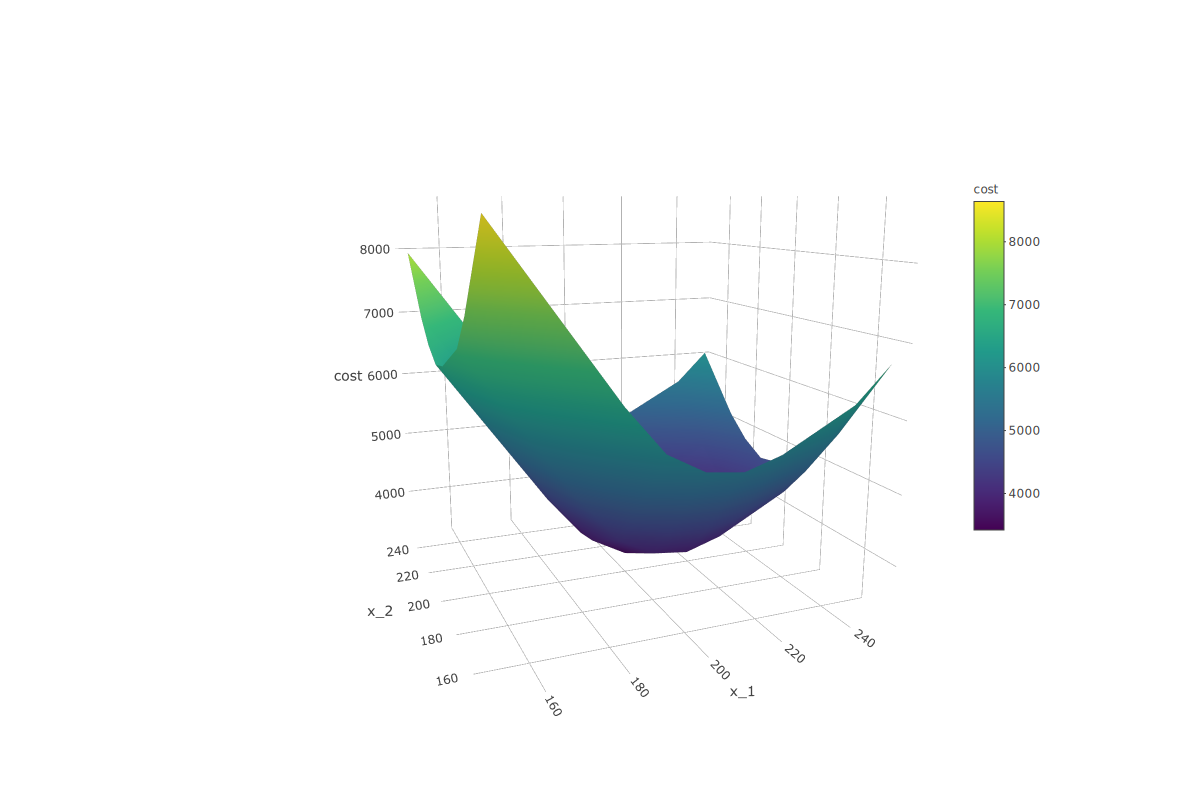
\includegraphics[width=0.8\textwidth]{Example-figure_files/figure-latex/3d cost.png}
\label{fig:3d}
\end{figure}

\begin{figure}[ht]
\centering
\caption{Contour of costs with boundaries}
\hspace{0.7cm}
\includegraphics[width=0.9\textwidth]{Example-figure_files/figure-latex/contour.png}
\label{fig:con}
\end{figure}

In Figure \ref{fig:con}, we also include two example boundaries to demonstrate different kinds of feasible region (on the left side of boundary). Moreover, we define a \emph{prime point} to denote the optimal solution when all constraints are relaxed. One can see that boundary 1 forms a feasible region contains the prime point, while the feasible region formed by boundary 2 doesn't. There is no doubt that the optimal solution for MPNP with boundary 1 is lying exactly at the prime point, and the solution will remains optimal as long as the prime point is not \say{pushed out} of the feasible region. On the other hand, one can easily show the optimal solution for MPNP with boundary 2 lies on the boundary since the cost function is convex \cite{DT06}, and the solution on this case is more sensitive. Costs on boundaries see Figure \ref{fig:bd1} and Figure \ref{fig:bd2} in Appendix \ref{se:costfun}.

Now, we consider the boundary for the example in Section \ref{se:sensitivity}. We have equation set:
\[
\begin{cases}
    4 x_1 + 6 x_2 \leq 2200\\
    7 x_1 + 5 x_2 \leq 2500\\
    8 x_1 + 8 x_2 \leq 3500,
\end{cases}
\]
that forms the boundary in Figure \ref{fig:conexam}. It is clear this feasible region doesn't include the prime point. Therefore, the optimal solution should lies on boundary, as we computed in Section \ref{se:sensitivity}. One can compare the relaxed solution, the prime point $\big( 210,210 \big)$, with the true optimal solution on boundary $\big( 207.1,210 \big)$.

\begin{figure}[ht]
\caption{Contour of cost with example boundary}
\hspace{1cm}
\includegraphics[width=0.9\textwidth]{Example-figure_files/figure-latex/conexam.png}
\label{fig:conexam}
\end{figure}

Moreover, we can visualise the effect on changes using contour plot. Any changes on demand distribution will lead to the move of prime point, and any changes on costs will lead to the change on the density of contour lines. For instance, if we apply the price-demand correlation, and decrease the under-stocking cost of product $a$ by 0.6, the prime point will moves to the right by $|0.6\,\beta|$, along with all contour lines, and the contour lines at the left side of prime point will become looser. See the contour plot after changes in Figure \ref{fig:newcon}.

\begin{figure}[ht]
\caption{Contour of cost after decreasing under-stocking cost}
\hspace{1cm}
\includegraphics[width=0.9\textwidth]{Example-figure_files/figure-latex/newcon.png}
\label{fig:newcon}
\end{figure}

One can see the optimal solution doesn't move. Actually, the optimal solution will remain optimal as long as $\Delta c_a^u \in \big[ -0.7,0.29 \big]$. Any changes below -0.7 will cause the optimal point moves along boundary, and any changes above 0.29 will \say{push in} the prime point. Similar results apply to product $b$. Simulation results see Figure \ref{fig:demandunder}.

\begin{figure}[ht]
\centering
\caption{Change of optimal cost given price-demand correlation}
\includegraphics{Example-figure_files/figure-latex/demandunder-1.pdf}
\label{fig:demandunder}
\end{figure}

Now, we derive the margin of $\Delta c_a^u$ providing the changes in allowable range.

We first define:
\[
    \Delta y_j^s =
    \begin{cases}
        -\Delta \mu_j, & y_j^s > 0,\\
        0, & y_j^s = 0,
    \end{cases}
\]
and,
\[
    \Delta z_j^s =
    \begin{cases}
        \Delta \mu_j, & z_j^s > 0,\\
        0, & z_j^s = 0.
    \end{cases}
\]
Thus:
\[
\begin{aligned}
    \Delta \, C_{c_{j'}^u}
    & = c_{j'}^o \Delta y_{j'} + \sum_{s \in S} \big[ \big( c_{j'}^u + \Delta c_{j'}^u \big) \big( z_{j'}^s + \Delta z_{j'}^s \big) - c_{j'}^u z_{j'}^s \big]\\
    & = -c_{j'}^o N_{j'}^o \Delta \mu_{j'} + c_{j'}^u 
    N_{j'}^u \Delta \mu_{j'} + \Delta c_{j'}^u \sum_{s \in S} z_{j'}^s + N_{j'}^u \Delta c_{j'}^u \Delta \mu_{j'}\\
    & = -c_{j'}^o N_{j'}^o \beta \Delta c_{j'}^u + c_{j'}^u N_{j'}^u \beta \Delta c_{j'}^u + \Delta c_{j'}^u \sum_{s \in S} z_{j'}^s + N_{j'}^u \Delta c_{j'}^u \beta \Delta c_{j'}^u\\
    & = N_{j'}^u \beta \big( \Delta c_{j'}^u \big)^2 + \big[ c_{j'}^u N_{j'}^u \beta - c_{j'}^o N_{j'}^o \beta + \sum_{s \in S} z_{j'}^s \big] \Delta c_{j'}^u.
\end{aligned}
\]
Putting $\beta$, $N_a^u$, $N_a^o$, $c_a^u$, $c_a^o$ and $z_a^s$ in, we have:
\[
    \Delta \, C_{c_a^u} = -60 \big( \Delta c_a^u \big)^2 + 67.14 \Delta c_a^u.
\]

In general, there exists a parabolic relationship between $\Delta \, C_{c_{j'}^u}$ and $\Delta c_{j'}^u$. Thus, we may apply features of parabolic function:
\begin{itemize}
    \item Point $(0,0)$ is on the parabola,
    \item Given $\beta < 0$, the parabola is opening to the bottom,
    \item The axis of parabola is positive when $\sum_{s \in S} z_{j'}^s > \beta \big( c_{j'}^o N_{j'}^o - c_{j'}^u N_{j'}^u \big)$.
\end{itemize}
Using these features, we could derive:
\begin{eqnarray}
\label{eq:condition}
    \frac{1}{|S|} \sum_{s \in S} z_{j'}^s > \frac{\beta \big( c_{j'}^o N_{j'}^o - c_{j'}^u N_{j'}^u \big)}{N_{j'}^o + N_{j'}^u} \implies \lim_{\Delta c_{j'}^u \to 0^-} \frac{\Delta \, C_{c_{j'}^u}}{\Delta c_{j'}^u} > 0
\end{eqnarray}
Recalling $\beta$ is the multiplier between mean demand and under-stocking cost, we may interpret (\ref{eq:condition}) as \say{One can reduce total cost by decreasing under-stocking cost of particular product when current under-stocking of that product is greater than expected over-stocking/under-stocking cost difference times the given multiplier.}





\section{Summary}
%\label{se:conclusion}
This paper provides a framework of applying LP sensitivity analysis on formulated MPNP. We first formulate the MPNP into a two-stage stochastic linear programming with recourse, which can be view as large LP model with finite scenarios. Then, we perform the classic sensitivity analysis to derive the shadow price/reduced cost. As long as the changes in allowable range, we can inform the market decision directly.

This method is very efficient since we don’t need to resolve the optimisation problem. We also perform an example to verify our result. The result from our method is in line with the simulation output.

Besides, we present one extension that consider correlated parameters. 

%%%%%%%%%%%%%%%%%%%%%%%%%%%%%%
\printbibliography
%%%%%%%%%%%%%%%%%%%%%%%%%%%%%%
\newpage
\begin{center}
{\bf\Large Appendices}
\end{center}

\appendix
\section{Sensitivity Report}
\label{se:report}

\begingroup\fontsize{7}{9}\selectfont
\begin{longtable}{cccccc}
\caption{Sensitivity Report: Variable Cells}
\label{tab:sen_var}\\
\toprule
variable & final value & reduced cost & coefficient & allowable increase & allowable decrease\\
\midrule
\endfirsthead
\multicolumn{6}{@{}l}{\textit{(continued)}}\\
\toprule
variable & final value & reduced cost & coefficient & allowable increase & allowable decrease\\
\midrule
\endhead
\
\endfoot
\bottomrule
\endlastfoot
$y_1^1$ & 7.1 & 0.0 & 5 & 6.0 & 3.8\\
$y_1^2$ & 0.0 & 5.0 & 5 & 10000.0 & 5.0\\
$y_1^3$ & 27.1 & 0.0 & 5 & 6.0 & 3.8\\
$y_1^4$ & 17.1 & 0.0 & 5 & 6.0 & 3.8\\
$y_1^5$ & 17.1 & 0.0 & 5 & 6.0 & 3.8\\
\addlinespace
$y_1^6$ & 0.0 & 5.0 & 5 & 10000.0 & 5.0\\
$y_1^7$ & 0.0 & 5.0 & 5 & 10000.0 & 5.0\\
$y_1^8$ & 0.0 & 5.0 & 5 & 10000.0 & 5.0\\
$y_1^9$ & 7.1 & 0.0 & 5 & 6.0 & 3.8\\
$y_1^{10}$ & 17.1 & 0.0 & 5 & 6.0 & 3.8\\
\addlinespace
$y_1^{11}$ & 0.0 & 5.0 & 5 & 10000.0 & 5.0\\
$y_1^{12}$ & 0.0 & 5.0 & 5 & 10000.0 & 5.0\\
$y_2^1$ & 0.0 & 7.0 & 7 & 10000.0 & 7.0\\
$y_2^2$ & 0.0 & 7.0 & 7 & 10000.0 & 7.0\\
$y_2^3$ & 10.0 & 0.0 & 7 & 2.7 & 4.3\\
\addlinespace
$y_2^4$ & 30.0 & 0.0 & 7 & 2.7 & 4.3\\
$y_2^5$ & 0.0 & 4.3 & 7 & 10000.0 & 4.3\\
$y_2^6$ & 0.0 & 7.0 & 7 & 10000.0 & 7.0\\
$y_2^7$ & 40.0 & 0.0 & 7 & 2.7 & 4.3\\
$y_2^8$ & 60.0 & 0.0 & 7 & 2.7 & 4.3\\
\addlinespace
$y_2^9$ & 30.0 & 0.0 & 7 & 2.7 & 4.3\\
$y_2^{10}$ & 0.0 & 7.0 & 7 & 10000.0 & 7.0\\
$y_2^{11}$ & 0.0 & 7.0 & 7 & 10000.0 & 7.0\\
$y_2^{12}$ & 0.0 & 7.0 & 7 & 10000.0 & 7.0\\
$z_1^1$ & 0.0 & 6.0 & 6 & 10000.0 & 6.0\\
\addlinespace
$z_1^2$ & 12.9 & 0.0 & 6 & 3.8 & 6.0\\
$z_1^3$ & 0.0 & 6.0 & 6 & 10000.0 & 6.0\\
$z_1^4$ & 0.0 & 6.0 & 6 & 10000.0 & 6.0\\
$z_1^5$ & 0.0 & 6.0 & 6 & 10000.0 & 6.0\\
$z_1^6$ & 2.9 & 0.0 & 6 & 3.8 & 6.0\\
\addlinespace
$z_1^7$ & 32.9 & 0.0 & 6 & 3.8 & 6.0\\
$z_1^8$ & 42.9 & 0.0 & 6 & 3.8 & 6.0\\
$z_1^9$ & 0.0 & 6.0 & 6 & 10000.0 & 6.0\\
$z_1^{10}$ & 0.0 & 6.0 & 6 & 10000.0 & 6.0\\
$z_1^{11}$ & 2.9 & 0.0 & 6 & 3.8 & 6.0\\
\addlinespace
$z_1^{12}$ & 32.9 & 0.0 & 6 & 3.8 & 6.0\\
$z_2^1$ & 40.0 & 0.0 & 6 & 4.3 & 2.7\\
$z_2^2$ & 20.0 & 0.0 & 6 & 4.3 & 2.7\\
$z_2^3$ & 0.0 & 6.0 & 6 & 10000.0 & 6.0\\
$z_2^4$ & 0.0 & 6.0 & 6 & 10000.0 & 6.0\\
\addlinespace
$z_2^5$ & 0.0 & 0.0 & 6 & 4.3 & 2.7\\
$z_2^6$ & 0.0 & 0.0 & 6 & 4.3 & 2.7\\
$z_2^7$ & 0.0 & 6.0 & 6 & 10000.0 & 6.0\\
$z_2^8$ & 0.0 & 6.0 & 6 & 10000.0 & 6.0\\
$z_2^9$ & 0.0 & 6.0 & 6 & 10000.0 & 6.0\\
\addlinespace
$z_2^{10}$ & 10.0 & 0.0 & 6 & 4.3 & 2.7\\
$z_2^{11}$ & 50.0 & 0.0 & 6 & 4.3 & 2.7\\
$z_2^{12}$ & 50.0 & 0.0 & 6 & 4.3 & 2.7\\
$x_1$ & 207.1 & 0.0 & 0 & 6.0 & 3.8\\
$x_2$ & 210.0 & 0.0 & 0 & 2.7 & 4.3\\*
\end{longtable}
\endgroup{}

\begingroup\fontsize{6}{9}\selectfont
\begin{longtable}{cccccc}
\caption{Sensitivity Report: Constraints}
\label{tab:sen_con}\\
\toprule
row & final value & shadow price & constraint RHS & allowable increase & allowable decrease\\
\midrule
\endfirsthead
\multicolumn{6}{@{}l}{\textit{(continued)}}\\
\toprule
row & final value & shadow price & constraint RHS & allowable increase & allowable decrease\\
\midrule
\endhead
\
\endfoot
\bottomrule
\endlastfoot
time\_A & 2088.6 & 0.0 & 2200 & 10000.0 & 111.4\\
time\_B & 2500.0 & -0.9 & 2500 & 20.0 & 50.0\\
time\_C & 3337.1 & 0.0 & 3500 & 10000.0 & 162.9\\
over\_1\textasciicircum{}1 & 200.0 & -5.0 & 200 & 7.1 & 10000.0\\
over\_1\textasciicircum{}2 & 207.1 & 0.0 & 220 & 10000.0 & 12.9\\
\addlinespace
over\_1\textasciicircum{}3 & 180.0 & -5.0 & 180 & 27.1 & 10000.0\\
over\_1\textasciicircum{}4 & 190.0 & -5.0 & 190 & 17.1 & 10000.0\\
over\_1\textasciicircum{}5 & 190.0 & -5.0 & 190 & 17.1 & 10000.0\\
over\_1\textasciicircum{}6 & 207.1 & 0.0 & 210 & 10000.0 & 2.9\\
over\_1\textasciicircum{}7 & 207.1 & 0.0 & 240 & 10000.0 & 32.9\\
\addlinespace
over\_1\textasciicircum{}8 & 207.1 & 0.0 & 250 & 10000.0 & 42.9\\
over\_1\textasciicircum{}9 & 200.0 & -5.0 & 200 & 7.1 & 10000.0\\
over\_1\textasciicircum{}10 & 190.0 & -5.0 & 190 & 17.1 & 10000.0\\
over\_1\textasciicircum{}11 & 207.1 & 0.0 & 210 & 10000.0 & 2.9\\
over\_1\textasciicircum{}12 & 207.1 & 0.0 & 240 & 10000.0 & 32.9\\
\addlinespace
under\_1\textasciicircum{}1 & 207.1 & 0.0 & 200 & 7.1 & 10000.0\\
under\_1\textasciicircum{}2 & 220.0 & 6.0 & 220 & 10000.0 & 12.9\\
under\_1\textasciicircum{}3 & 207.1 & 0.0 & 180 & 27.1 & 10000.0\\
under\_1\textasciicircum{}4 & 207.1 & 0.0 & 190 & 17.1 & 10000.0\\
under\_1\textasciicircum{}5 & 207.1 & 0.0 & 190 & 17.1 & 10000.0\\
\addlinespace
under\_1\textasciicircum{}6 & 210.0 & 6.0 & 210 & 10000.0 & 2.9\\
under\_1\textasciicircum{}7 & 240.0 & 6.0 & 240 & 10000.0 & 32.9\\
under\_1\textasciicircum{}8 & 250.0 & 6.0 & 250 & 10000.0 & 42.9\\
under\_1\textasciicircum{}9 & 207.1 & 0.0 & 200 & 7.1 & 10000.0\\
under\_1\textasciicircum{}10 & 207.1 & 0.0 & 190 & 17.1 & 10000.0\\
\addlinespace
under\_1\textasciicircum{}11 & 210.0 & 6.0 & 210 & 10000.0 & 2.9\\
under\_1\textasciicircum{}12 & 240.0 & 6.0 & 240 & 10000.0 & 32.9\\
over\_2\textasciicircum{}1 & 210.0 & 0.0 & 250 & 10000.0 & 40.0\\
over\_2\textasciicircum{}2 & 210.0 & 0.0 & 230 & 10000.0 & 20.0\\
over\_2\textasciicircum{}3 & 200.0 & -7.0 & 200 & 10.0 & 10000.0\\
\addlinespace
over\_2\textasciicircum{}4 & 180.0 & -7.0 & 180 & 30.0 & 10000.0\\
over\_2\textasciicircum{}5 & 210.0 & -2.7 & 210 & 0.0 & 4.0\\
over\_2\textasciicircum{}6 & 210.0 & 0.0 & 210 & 10000.0 & 0.0\\
over\_2\textasciicircum{}7 & 170.0 & -7.0 & 170 & 40.0 & 10000.0\\
over\_2\textasciicircum{}8 & 150.0 & -7.0 & 150 & 60.0 & 10000.0\\
\addlinespace
over\_2\textasciicircum{}9 & 180.0 & -7.0 & 180 & 30.0 & 10000.0\\
over\_2\textasciicircum{}10 & 210.0 & 0.0 & 220 & 10000.0 & 10.0\\
over\_2\textasciicircum{}11 & 210.0 & 0.0 & 260 & 10000.0 & 50.0\\
over\_2\textasciicircum{}12 & 210.0 & 0.0 & 260 & 10000.0 & 50.0\\
under\_2\textasciicircum{}1 & 250.0 & 6.0 & 250 & 10000.0 & 40.0\\
\addlinespace
under\_2\textasciicircum{}2 & 230.0 & 6.0 & 230 & 10000.0 & 20.0\\
under\_2\textasciicircum{}3 & 210.0 & 0.0 & 200 & 10.0 & 10000.0\\
under\_2\textasciicircum{}4 & 210.0 & 0.0 & 180 & 30.0 & 10000.0\\
under\_2\textasciicircum{}5 & 210.0 & 6.0 & 210 & 10000.0 & 0.0\\
under\_2\textasciicircum{}6 & 210.0 & 6.0 & 210 & 10000.0 & 0.0\\
\addlinespace
under\_2\textasciicircum{}7 & 210.0 & 0.0 & 170 & 40.0 & 10000.0\\
under\_2\textasciicircum{}8 & 210.0 & 0.0 & 150 & 60.0 & 10000.0\\
under\_2\textasciicircum{}9 & 210.0 & 0.0 & 180 & 30.0 & 10000.0\\
under\_2\textasciicircum{}10 & 220.0 & 6.0 & 220 & 10000.0 & 10.0\\
under\_2\textasciicircum{}11 & 260.0 & 6.0 & 260 & 10000.0 & 50.0\\
\addlinespace
under\_2\textasciicircum{}12 & 260.0 & 6.0 & 260 & 10000.0 & 50.0\\*
\end{longtable}
\endgroup{}

\section{Costs on boundaries}
\label{se:costfun}

\begin{figure}[ht]
\centering
\caption{Costs on boundary 1}
\includegraphics[width=\textwidth]{Example-figure_files/figure-latex/boundary1.png}
\label{fig:bd1}
\end{figure}

\begin{figure}[ht]
\centering
\caption{Costs on boundary 2}
\includegraphics[width=\textwidth]{Example-figure_files/figure-latex/boundary2.png}
\label{fig:bd2}
\end{figure}


\end{document}
